\documentclass[12pt]{article}

\usepackage{arxiv}
\usepackage[utf8]{inputenc} % allow utf-8 input
\usepackage[T1]{fontenc}    % use 8-bit T1 fonts
\usepackage{hyperref}       % hyperlinks
\usepackage{booktabs}       % professional-quality tables
\usepackage{amsfonts}       % blackboard math symbols
\usepackage{nicefrac}       % compact symbols for 1/2, etc.
\usepackage{microtype}      % micro typography
\usepackage{lipsum}
\usepackage{fancyhdr}       % header
\usepackage{graphicx}       % graphics
\usepackage{lineno}
\usepackage{setspace}

\singlespacing
\graphicspath{{figure/}}     % organize figures under figure/ folder

\pagestyle{fancy}
\thispagestyle{empty}
\rhead{ \textit{ }} 
% \fancyhead[LO]{Running Title for Header}

\title{A template for Arxiv Style Papers}

\author{
  Author A \\
  Department of BCD \\
  EFG University \\
  HIJ, China \\
  \texttt{email@main.com} \\
  \And
  Author B \\
  Department of BCD \\
  EFG University \\
  HIJ, China \\
  \texttt{email@main.com} \\
  \And
  Author C \\
  Department of BCD \\
  EFG University \\
  HIJ, China \\
  \texttt{email@main.com} \\
}

\begin{document}
\maketitle
% \linenumbers

% text
\begin{abstract}
This is the abstract. 
\end{abstract}

\keywords{First keyword \and Second keyword \and More}

\section{Introduction}\label{sec:introduction}

This is the introduction. 

This paper is organized as follows. Section~\ref{sec:review} reviews related literature. Section~\ref{sec:method} formulates the proposed method. Section~\ref{sec:data} describes the dataset. Section~\ref{sec:results} discusses the results. Section~\ref{sec:conclusion} concludes this paper.


\section{Literature Review}\label{sec:review}

Text~\cite{kour2014real,kour2014fast} and see~\cite{hadash2018estimate}.

\subsection{Headings: second level}

Text with second level heading.

\subsubsection{Headings: third level}

Text with third level heading.

\paragraph{Paragraph}

Text with fourth level heading.

\section{Methodology}\label{sec:method}

\subsection{Formulas}

As expressed by Equation~\ref{eq:formula}.
\begin{equation}
    \label{eq:formula}
    \xi _{ij}(t)=P(x_{t}=i,x_{t+1}=j|y,v,w;\theta)= {\frac {\alpha _{i}(t)a^{w_t}_{ij}\beta _{j}(t+1)b^{v_{t+1}}_{j}(y_{t+1})}{\sum _{i=1}^{N} \sum _{j=1}^{N} \alpha _{i}(t)a^{w_t}_{ij}\beta _{j}(t+1)b^{v_{t+1}}_{j}(y_{t+1})}}
\end{equation}

\subsection{Figures}

See Figure~\ref{fig:fig1}.

\subsection{Tables}

See awesome Table~\ref{tab:table}.

\section{Data}\label{sec:data}

Describe the dataset used in the study, including its source, characteristics, and any preprocessing steps taken before analysis.
\section{Results and Discussion}\label{sec:results}

Results and discussion go here.
\section{Conclusion}\label{sec:conclusion}

Your conclusion here.


% table and figure
% table sample
\begin{table}
 \caption{Sample table title}
  \centering
  \begin{tabular}{lll}
    \toprule
    \multicolumn{2}{c}{Part}                   \\
    \cmidrule(r){1-2}
    Name     & Description     & Size ($\mu$m) \\
    \midrule
    Dendrite & Input terminal  & $\sim$100     \\
    Axon     & Output terminal & $\sim$10      \\
    Soma     & Cell body       & up to $10^6$  \\
    \bottomrule
  \end{tabular}
\label{tab:table}
\end{table}
% figure sample 
\begin{figure}
  \centering
  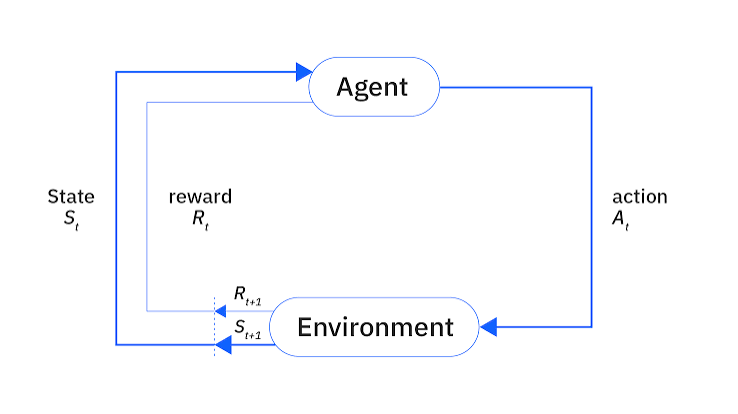
\includegraphics[width=0.8\linewidth]{images.png}
  \caption{Sample figure caption.}
  \label{fig:fig1}
\end{figure}

\section*{Acknowledgments}
This work was supported in part by.

\bibliographystyle{unsrt}
\bibliography{references}

\end{document}
